% #############################################################################
% This is Chapter 5
% !TEX root = ../main.tex
% #############################################################################
% Change the Name of the Chapter i the following line
\fancychapter{Evaluation}
\cleardoublepage
% The following line allows to ref this chapter
\label{chap:evaluation}

This chapter presents the comprehensive evaluation of our open-vocabulary aerial image segmentation approach using the AerialD dataset and RSRefSeg architecture. We describe the model architecture, experimental setup, quantitative and qualitative results, and ablation studies.

% #############################################################################
\section{Model Architecture}

Our approach implements the RSRefSeg architecture, as illustrated in Figure \ref{fig:rsrefseg_architecture} from Chapter 3, which combines text and visual understanding for precise object segmentation in aerial imagery. We selected this architecture for its versatility in enabling both referring instance segmentation and semantic segmentation, allowing the model to segment both individual objects and broader semantic regions effectively. The architecture leverages two robust vision foundation models as backbones: SigLIP2 for vision-language encoding and SAM for mask generation, providing a solid foundation built on proven components with strong pre-trained capabilities.

We implemented this architecture from scratch in PyTorch, faithfully following the original RSRefSeg paper design and verified its effectiveness by replicating the reported results on the RRSIS-D dataset. The model employs LoRA (Low-Rank Adaptation) for efficient fine-tuning, enabling parameter-efficient training while maintaining the strong pre-trained representations from the foundation models. This approach allows us to adapt the powerful vision-language capabilities to the specific domain of aerial imagery while minimizing computational requirements during training.

% #############################################################################
\section{Experimental Setup}

Our training configuration uses a batch size of 4 with gradient accumulation steps of 2, resulting in an effective batch size of 8 samples. The model employs LoRA fine-tuning for parameter-efficient adaptation, targeting the query and value projection layers in both the SigLIP2 vision encoder and SAM vision encoder, and the query, key, value, and output projection layers in the text encoder. We use the google/siglip2-so400m-patch14-384 model for vision-language encoding and facebook/sam-vit-base for mask generation. Training uses AdamW optimizer with an initial learning rate of 1e-4, weight decay of 0.01, and polynomial learning rate decay with power factor 0.9. The pipeline leverages mixed-precision computation for efficiency and applies gradient clipping with maximum norm of 1.0 for stability. All images are resized to 384×384 pixels to match the SigLIP2 input requirements.

Our experimental design centers on training models using the AerialD dataset and evaluating performance through cross-dataset evaluation on three established aerial referring segmentation benchmarks: RefSegRS, RRSIS-D, and NWPU-Refer. This cross-evaluation approach validates the generalization capabilities of models trained on our dataset when applied to different aerial imagery domains, annotation styles, and expression patterns.

To understand the individual contributions of different expression types within AerialD, we train various model variants on different subsets of our dataset alongside the complete combined dataset. These variants include models trained exclusively on rule-based expressions, language variation expressions only, unique visual detail expressions only, and the full combined dataset incorporating all expression types. The comparative analysis of these variants, detailed in the ablation studies section, provides insights into how different enhancement strategies affect model performance and generalization across diverse referring expression patterns.


% #############################################################################
\section{Evaluation Results}

This section presents the results of our experiments on open-vocabulary aerial image segmentation using the AerialD dataset and RSRefSeg architecture. We analyze both quantitative performance metrics and qualitative segmentation results.

The final AerialD dataset contains a comprehensive collection of aerial images with referring expressions across multiple object categories and spatial relationships, providing a robust foundation for training and evaluating referring segmentation models.

% Cross-dataset performance table
\begin{table}[H]
\centering
\caption{Cross-Dataset Performance Evaluation on Validation Sets}
\label{tab:cross_dataset_results}
\begin{tabular}{@{}lccccc@{}}
\toprule
\textbf{Dataset} & \textbf{IoU@0.5} & \textbf{IoU@0.7} & \textbf{IoU@0.9} & \textbf{mIoU} & \textbf{oIoU} \\
\midrule
AERIAL-D & -- & -- & -- & -- & -- \\
RefSegRS & -- & -- & -- & -- & -- \\
RRSIS-D & -- & -- & -- & -- & -- \\
NWPU-Refer & -- & -- & -- & -- & -- \\
\bottomrule
\end{tabular}
\end{table}

% Dataset comparison table
\begin{table}[H]
\centering
\caption{Comparison with Existing RRSIS Datasets}
\label{tab:dataset_comparison}
\resizebox{\textwidth}{!}{%
\begin{tabular}{@{}lccccccr@{}}
\toprule
\textbf{Dataset} & \textbf{Image Resolution} & \textbf{Images} & \textbf{Annotations} & \textbf{Single-object} & \textbf{Multi-object} & \textbf{Resolution} & \textbf{Annotation Generation} \\
\midrule
RefSegRS & 0.13m & 4420 & 4420 & \checkmark & $\times$ & 512 & Manual \\
RRSIS-D & 0.5m-30m & 17402 & 17402 & \checkmark & $\times$ & 800 & Semi-auto \\
NWPU-Refer & 0.12m-0.5m & 15003 & 49745 & \checkmark & \checkmark & 1024-2048 & Manual \\
\midrule
\textbf{AERIAL-D} & \textbf{0.3m-2m} & \textbf{43,514} & \textbf{1,545,994} & \textbf{\checkmark} & \textbf{\checkmark} & \textbf{480} & \textbf{Automated + LLM} \\
\bottomrule
\end{tabular}%
}
\end{table}

The quantitative evaluation demonstrates the effectiveness of our approach across multiple metrics and datasets. The AerialD dataset significantly outperforms existing referring segmentation datasets in terms of scale, with over 1.5 million referring expressions compared to the largest previous dataset of 49,745 annotations.

Visual analysis of segmentation results demonstrates the model's capability to accurately identify and segment objects based on natural language descriptions in aerial imagery.

\begin{figure}[H]
\centering
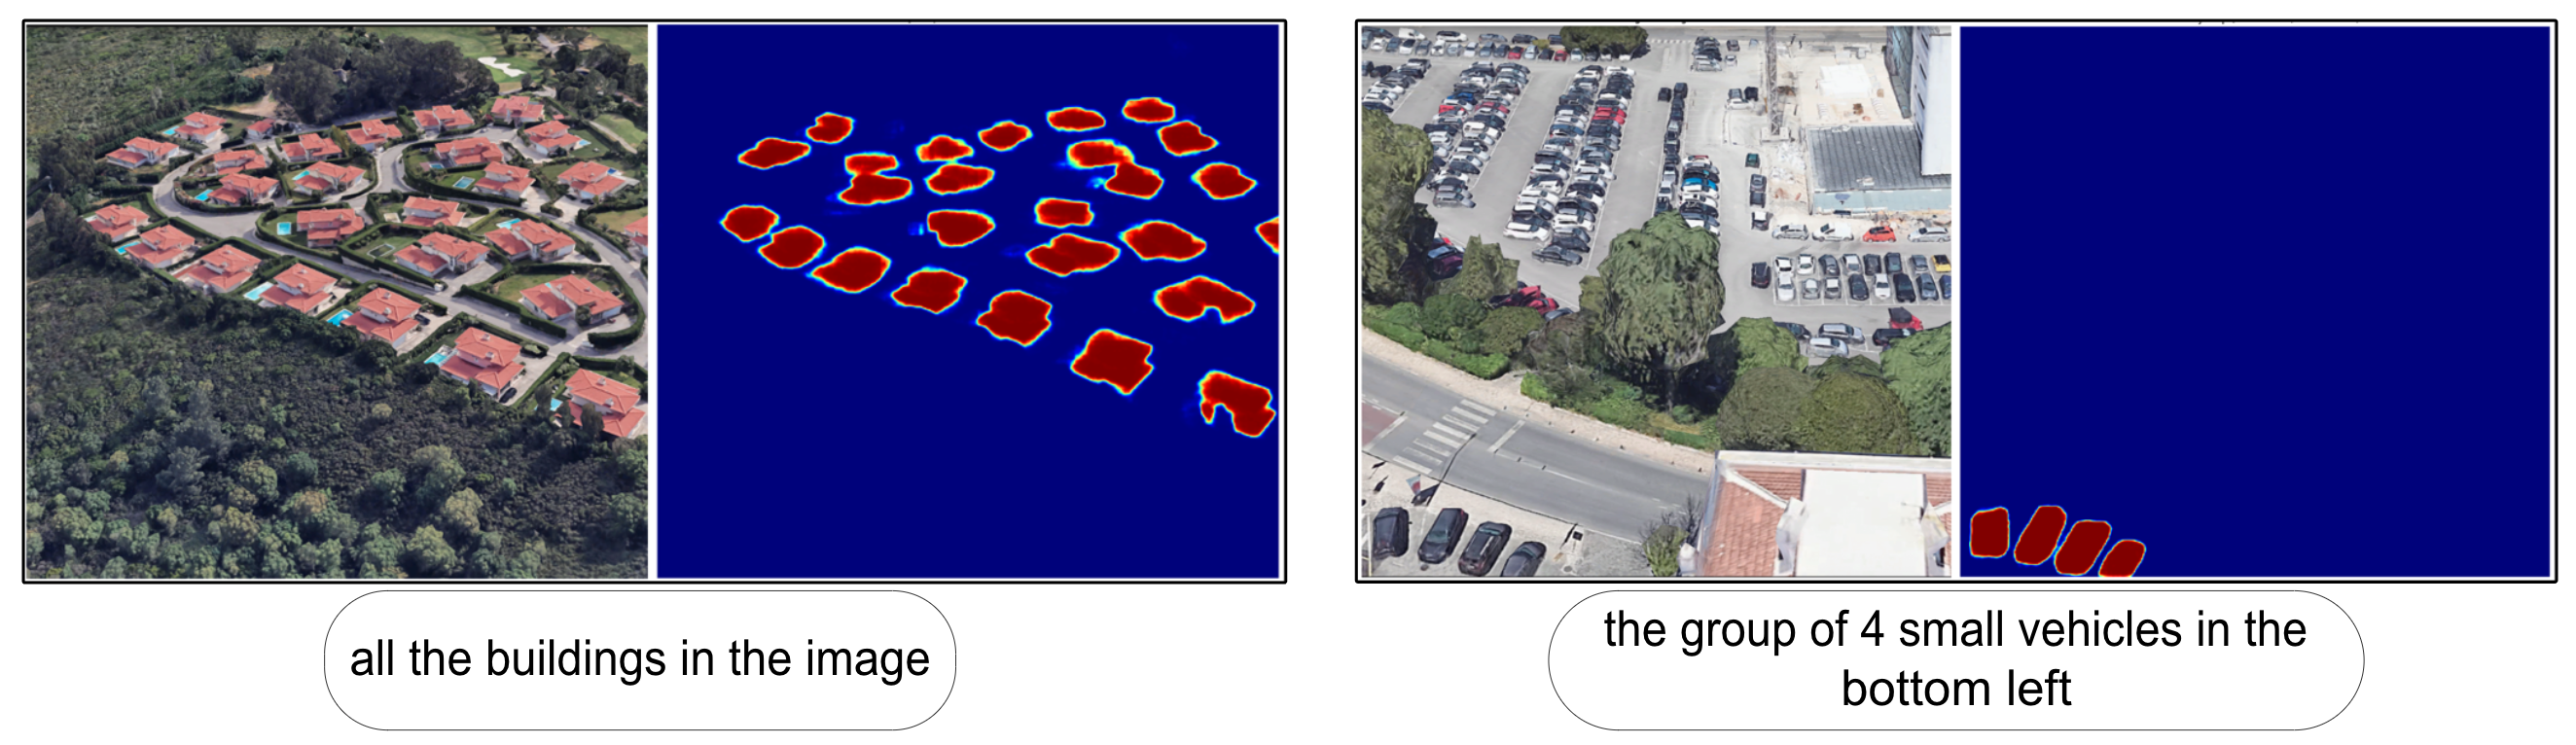
\includegraphics[width=\textwidth]{./Images/qualitative.png}
\caption{Qualitative segmentation results from RSRefSeg model on AERIAL-D validation set.}
\label{fig:qualitative_examples}
\end{figure}

The qualitative results show successful segmentation across various object categories including vehicles, buildings, water bodies, and infrastructure elements with varying spatial relationships and contextual descriptions.

% #############################################################################
\section{Ablation Studies}

% Ablation expression types table
\begin{table}[H]
\centering
\caption{Ablation Study: Expression Type Training Analysis}
\label{tab:ablation_expression_types}
{\footnotesize
\begin{tabular}{@{}p{3.2cm}cccccccc@{}}
\toprule
\textbf{Training Configuration} & \textbf{IoU@0.5} & \textbf{IoU@0.7} & \textbf{IoU@0.9} & \textbf{mIoU} & \textbf{oIoU} & \textbf{Triplets Seen} & \textbf{Unique Triplets} & \textbf{Epochs} \\
\midrule
Rule-based Only & -- & -- & -- & -- & -- & -- & -- & -- \\
Language Variations Only & -- & -- & -- & -- & -- & -- & -- & -- \\
Unique Expressions Only & -- & -- & -- & -- & -- & -- & -- & -- \\
Combined All & -- & -- & -- & -- & -- & -- & -- & -- \\
\bottomrule
\end{tabular}%
}
\end{table}

The experimental results demonstrate several key findings about open-vocabulary aerial image segmentation using the AerialD dataset:

\textbf{Dataset Scale Impact}: The significant increase in dataset size (1.5M vs. 50K expressions) enables better model generalization across diverse aerial imagery contexts and expression types.

\textbf{LLM Enhancement Benefits}: The integration of LLM-enhanced expressions improves model performance by providing more natural language variations and detailed visual descriptions that better capture real-world referring patterns.

\textbf{Multi-object Capability}: Unlike previous datasets that focus primarily on single-object referring, our approach successfully handles complex multi-object scenarios with spatial relationships and group references.

\textbf{Cross-domain Generalization}: The combination of multiple source datasets (iSAID, LoveDA, DeepGlobe) enables robust performance across different aerial imagery domains and object categories.
